\documentclass[12pt]{report}

\usepackage[T1]{fontenc}
\usepackage[utf8]{inputenc}
\usepackage{graphicx}

\begin{document}

\begin{center}
{\Huge \textbf{Modulacion de ancho de pulso .}\\}
\Large{Enesto Alonso Partida López\\ Universidad Politecnica De La Zona Metropolitana De Guadalajara\\ Mecatronica 4 A\\ Septiembre-diciembre 2019}\\
{22 de octubre 2019 }\\
\end{center}
\begin{center}



\includegraphics[scale=1]{../../../../Downloads/upzmg.jpg} 
\end{center}
\newpage
{\huge \textbf{¿Que es un PWM?}\\}


{\Large Tipo de señal de voltaje utilizada para enviar información o para modificar la cantidad de energía que se envía a una carga. Este tipo de señales es muy utilizada en circuitos digitales que necesitan emular una señal analógica.\\
Este tipo de señales son de tipo cuadrada o sinusiodales en las cuales se les cambia el ancho relativo respecto al período de la misma, el resultado de este cambio es llamado ciclo de trabajo y sus unidades están representadas en términos de porcentaje. }\\

\begin{center}
\begin{figure}[hbtp]
\centering
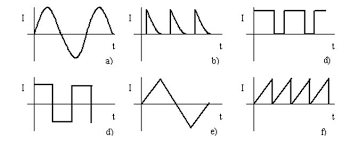
\includegraphics[scale=1]{../../../../Downloads/descragas/pwm.png}
\caption{Señales PWM}
\end{figure}

\end{center}
{\huge \textbf{¿Cómo se construye un circuito PWM?  }}\\

{\Large Se lleva a cabo mediante un comparador con dos entradas y una salida. Una de las entradas se conecta a un oscilador de onda triangular, mientras que la otra queda disponible para la señal moduladora. En la salida la frecuencia es generalmente igual a la de la señal triangular y el ciclo de trabajo está en función de la portadora. }\\
\begin{center}
\begin{figure}[hbtp]
\caption{Circuito PWM con 555}
\centering
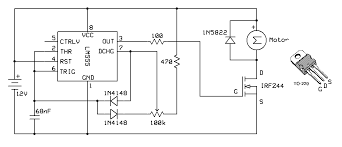
\includegraphics[scale=1.1]{../../../../Downloads/descragas/circuito.png}
\end{figure}

\end{center}
{\Large La modulación por ancho de pulsos es una técnica utilizada para regular la
velocidad de giro de los motores eléctricos. Mantiene el par motor constante y
no supone un desaprovechamiento de la energía eléctrica. Se utiliza tanto en
corriente continua como en alterna.\\Otra forma de regular el giro del motor es variando el tiempo entre pulsos modulación por frecuencia de pulsos de duración constante.}\\\\
{\huge \textbf{Aplicaciones }}\\

{\Large Las aplicaciones típicas para este tipo de señales son: Controlar intensidad de un LED, mover servomotores, controlar LED RGB, controlar velocidad de motores de corriente continua y controlar motores eléctricos de inducción o asincrónicos. }\\
\begin{center}
\begin{figure}[hbtp]
\caption{Funcionamiento y onda de un PWM}
\centering
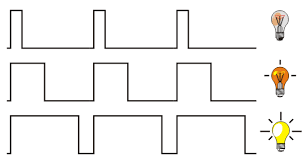
\includegraphics[scale=1]{../../../../Downloads/descragas/images.png}
\end{figure}

\end{center}

{\huge \textbf{Principal desventaja}\\
{\Large La posibilidad de que haya interferencias generadas por
radiofrecuencia. Estas pueden minimizarse mediante el uso de un
microcontrolador ubicado cerca de la carga y realizando un filtrado de la fuente
de alimentación}
\newpage
{\huge \textbf{Bibliografia:}\\}\\
{\large
@online{Electronica Unicrom,
author = {CRUZ CUEVAS JENNYFER,
MONTESINOS DE LA ROSA EDGAR ENRIQUE,
SANTANA ROBLES JONATHAN},
title = {“GENERADOR DE SEÑALES PARA CIRCUITOS
 DE ELECTRÓNICA DE POTENCIA”},
year = {2010},
url = {https://tesis.ipn.mx/jspui/bitstream/123456789/5702/1/GENERADORSENALES.pdf},
OPTsubtitle = {CIRCUITO GENERADOR
DE PULSOS
MODULADOS POR ANCHURA
OPTversion = {copyright},
OPTdate = {32},
OPTmonth = {1},

}
}

\end{document}